%! alt The robot's path from O: six moves of 1 metre, starting north, with turns of 100 and 140 degrees clockwise in turn. P1 to P5 are its positions after 1 to 5 moves, and the sixth move ends at O. The moves meet at P1 at an angle of 80 degrees. The points O, P2 and P4, reached after 0, 2 and 4 moves, form an equilateral triangle with side 2 sin 40 degrees, drawn dashed with its sides highlighted, because each pair of moves is the previous pair rotated by 120 degrees.
%! after_paragraph 1
%! scale 5
% The shared preamble of every Cevian figure. pipeline/figures turns these colours into theme-aware paint,
% and refuses any other colour, so draw only with them:
%   figink (lines and labels), figaux (construction lines), figaccent (the object the argument turns on),
%   figtint and figaccenttint (light fills).
\documentclass[border=1.5pt]{standalone}
\usepackage{tkz-euclide}
\definecolor{figink}{RGB}{0,0,0}
\definecolor{figaux}{RGB}{85,85,85}
\definecolor{figaccent}{RGB}{192,57,43}
\definecolor{figtint}{RGB}{221,221,221}
\definecolor{figaccenttint}{RGB}{245,213,208}
% tkz-euclide's defaults draw circles, compasses and marks in 50% grey and fill points with a tint.
\makeatletter
\def\tkz@otherlinecolor{figink}
\def\tkz@euc@circlecolor{figink}
\def\tkz@euc@compasscolor{figink}
\def\tkz@euc@mkcolor{figink}
\def\tkz@mk@fill{figink}
\def\tkz@euc@pointfillcolor{figink}
\makeatother
\tkzSetUpLine[color=figink,line width=.7pt]
\tkzSetUpArc[color=figink,line width=.7pt]
\tkzSetUpCompass[color=figink,line width=.5pt]
\tkzSetUpPoint[color=figink,fill=figink,size=3.1pt]
\tikzset{
  every picture/.style={line cap=round,line join=round,color=figink},
  circle style/.append style={color=figink,line width=.7pt},
  aux/.style={color=figaux,line width=.45pt,dash pattern=on 2.6pt off 2pt},
  key/.style={color=figaccent,line width=1pt},
  mk/.style={color=figink,line width=.5pt},
  lbl/.style={color=figink,inner sep=2.2pt},
  len/.style={color=figink,inner sep=1.5pt,font=\small},
}

\begin{document}
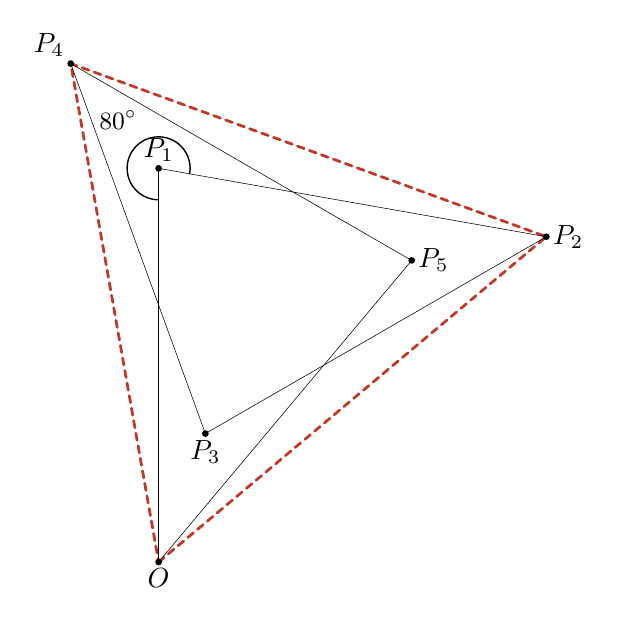
\begin{tikzpicture}
\tkzDefPoint(0.0,0.0){O} %! O = (0, 0)
\tkzDefPoint(0.000000000000000000000000000000000000000000000000010837084,5.0000000){P1} %! P1 = polar(O, 1, 90)
\tkzDefPoint(4.9240388,4.1317591){P2} %! P2 = polar(P1, 1, -10)
\tkzDefPoint(0.59391175,1.6317591){P3} %! P3 = polar(P2, 1, -150)
\tkzDefPoint(-1.1161890,6.3302222){P4} %! P4 = polar(P3, 1, 110)
\tkzDefPoint(3.2139380,3.8302222){P5} %! P5 = polar(P4, 1, -30)
%! fact dist(O, P1) == 1
%! fact dist(P5, O) == 1
%! fact angle(O, P1, P2) == 80
%! fact dist(O, P2) == 2*sind(40)
%! fact equal(dist(O, P2), dist(P2, P4))
%! fact equal(dist(P2, P4), dist(P4, O))
\tkzDrawPolygon[key,dash pattern=on 2.6pt off 2pt](O,P2,P4)
\tkzDrawSegments(O,P1 P1,P2 P2,P3 P3,P4 P4,P5 P5,O)
\tkzMarkAngle[size=.4,arc=l,mark=none,mk](P2,P1,O)
\tkzLabelAngle[pos=.8,font=\small](P2,P1,O){$80^\circ$}
\tkzDrawPoints(O,P1,P2,P3,P4,P5)
\tkzLabelPoint[below,lbl](O){$O$}
\tkzLabelPoint[above,lbl](P1){$P_1$}
\tkzLabelPoint[right,lbl](P2){$P_2$}
\tkzLabelPoint[below,lbl](P3){$P_3$}
\tkzLabelPoint[above left,lbl](P4){$P_4$}
\tkzLabelPoint[right,lbl](P5){$P_5$}
\end{tikzpicture}
\end{document}
